\documentclass[10pt]{article}

\usepackage[utf8]{inputenc}
\usepackage{geometry}
\geometry{top=2cm, bottom=2cm, left=1.5cm, right=1.5cm}
\usepackage{graphicx,graphics}
\usepackage[spanish, es-tabla]{babel}
\usepackage{hyperref}
\usepackage{graphicx}
\usepackage{url}
\usepackage{float}
\usepackage{amsmath}
\usepackage{multicol}
\usepackage{amssymb}
\usepackage{multirow}
\usepackage{gensymb}
\usepackage[center]{titlesec}
\usepackage[table,xcdraw]{xcolor}
\spanishdecimal{,}
\setlength{\parskip}{0mm}
\renewcommand{\thesection}{\large\Roman{section}}
\renewcommand{\thesubsection}{\large\Alph{subsection}}

\providecommand{\abs}[1]{\lvert#1\rvert}

%Título
\title{\textbf{Determinación experimental de la constante J para la transferencia de calor; ``Experimento de Joule"}}
\author{\normalsize{\emph{Andrés F. Valencia Fonseca}$^{1}$, \emph{Nicolás Aguilera García}$^{2}$}\\
\normalsize{\emph{Departamento de Física, Universidad del Valle, Cali, Colombia}}\\
\small{$^{1}$2125166, $^{2}$21273030}}
\date{(\small 20 de mayode 2023)}

\begin{document}

\maketitle
\begin{abstract}
En esta práctica, el objetivo es determinar la constante $J$ para la transferencia de calor en un sistema utilizando un calorímetro y una resistencia eléctrica. Se mide el cambio de temperatura para calcular la energía transferida en forma de calor, y a través de la realización de cuatro experimentos con diferentes condiciones iniciales, se obtuvieron datos de energía absorbida y energía transferida. Se aplicó una regresión lineal a los datos para determinar la constante $J$ experimental en cada caso. Sin embargo, se identificaron algunas fallas en el experimento, como posibles errores en las mediciones de masa, temperatura y corriente eléctrica, así como fugas de calor en el sistema. A pesar de estas limitaciones, se obtuvieron resultados cercanos al valor teórico esperado para la constante $J$. Los valores experimentales oscilan alrededor de $4.24$, con 
 un error porcentual de aproximadamente $1.5\%$. 
 Estos hallazgos contribuyen a una mejor comprensión de los fenómenos termodinámicos y la transferencia de energía en sistemas térmicos.
\end{abstract}
\begin{multicols*}{2}



\section{\small INTRODUCCIÓN}
En este experimento, nos enfocamos en analizar el efecto termodinámico de la corriente eléctrica aplicada a una resistencia sumergida en un calorímetro con agua. El objetivo es comprender cómo se produce la transferencia de energía en forma de calor y determinar experimentalmente la constante de proporcionalidad que relaciona el calor absorbido con la energía transferida.\\


Cuando la corriente eléctrica fluye a través de la resistencia calefactora, parte de la energía eléctrica se convierte en energía térmica, calentando así el agua presente en el vaso, a esto se denomina efecto Joule. El efecto Joule establece que la potencia disipada en una resistencia eléctrica es proporcional al cuadrado de la corriente que la atraviesa. Matemáticamente, esta relación se expresa mediante la siguiente ecuación:

\begin{equation}
\begin{split}
    P = I^2 R \\
    P = VI
    \label{Potencia}
\end{split}
\end{equation}

Donde $P$ representa la potencia disipada, $I$ es la corriente eléctrica, y $V$ la caída de potencial a través de la resistencia R.\\


La energía cedida en un tiempo $t$, considerando que la potencia $P$ es constante, se modela;
\begin{equation}
    E = Pt
    \label{Energia exp}
\end{equation}

Donde la energía $E$, está en Joules. De otra forma podemos calcular esta misma cantidad física considerando la conservación de la energía, dado que la energía $E$ que es disipada es absorbida por una cantidad $m$ de agua en el calorímetro, en forma de calor $\Delta Q$ tenemos que;

\begin{equation}
    E = J \Delta Q
    \label{Energia teorica}
\end{equation}

Dond $J$ es una constante de proporcionalidad entre el cambio de calor absorbido y la energía transferida al sistema,
esta constante será nuestro objeto de estudio a determinar, para ello es necesario calcular el calor $\Delta Q$. Puesto que el sistema de masa $M$ presenta un cambio de temperatura $\Delta T$, la energía transferida en forma de calor es;

\begin{equation}
    \Delta Q = (m_{cal} c_{cal} \,+ M_{agua}C_{agua})c\Delta T
    \label{Calor}
\end{equation}


El cambio de temperatura $\Delta T$ se refiere a la diferencia entre la temperatura final y la inicial del agua $T_f-T_0$.\\

Se realizarán mediciones de la temperatura del agua, a medida que se aplica una corriente eléctrica a la resistencia. A partir de estos datos, se calcula la cantidad de calor absorbido por el agua utilizando la ecuación \ref{Calor}. Y en paralelo, conociendo la potencia disipada \ref{Potencia}, a través del tiempo, desde las constantes de voltaje y corriente, podemos calcular la energía transferida por medio de la ecuación de la energía que relaciona estas variables \ref{Energia exp}. Luego, mediante una regresión lineal de los datos bajo la expresión \ref{Energia teorica}, se logra determinar el valor experimental de la constante J.\\

 La determinación de J a partir de los datos experimentales permitirá contrastar este valor con el teórico establecido para el agua, que es de aproximadamente 4.18 J/g·°C.


\section{\small METODOLOGÍA}

Para llevar a cabo el experimento, se preparó el sistema experimental (ver \textit{Figura \ref{montaje}}) que consistió en un calorímetro con agua y un circuito eléctrico con una resistencia calefactora $R$. Se comenzó pesando el calorímetro vacío y registrando su masa en la tabla de datos. Luego, se vertió una cantidad conocida de agua en el calorímetro y se anotó la masa del agua.\\
\begin{figure}[H]
    \centering
    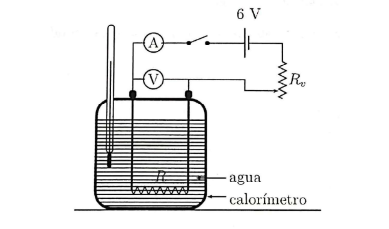
\includegraphics[scale=0.7]{montaje.png}
    \caption{Esquema del montaje experimental}
    \label{montaje}
\end{figure}
A continuación, se colocó la resistencia calefactora dentro del calorímetro con agua. Se utilizó un reóstato para ajustar la intensidad de la corriente eléctrica entre 2 A y 3 A, y se registraron los valores de corriente y voltaje a través de la resistencia.\\

Se procedió a medir la temperatura del agua utilizando un termómetro. Se aseguró de que el termómetro no estuviera en contacto directo con la resistencia calefactora para evitar interferencias en las mediciones de temperatura. Se tomó la temperatura inicial $T_0$ del agua como punto de partida para el experimento.\\

Una vez que el sistema estaba listo, se encendió el cronómetro y se registró el tiempo necesario para que la temperatura del agua cambiara. Se tomaron varios datos de temperatura y tiempo durante el proceso y se registraron en la tabla de datos.\\

Este proceso experimental se repitió 4 veces, para cantidades de masa de agua $M_{agua}$, corrientes $I$, y voltajes $V$, distintos, con el fin de reducir el error, y además para demostrar que dicha constante no depende de valores fijos de corriente o cantidad de agua, sino que es una propiedad extensiva.


\section{\small ANÁLISIS Y RESULTADOS}

Las condiciones iniciales de cada experimento, se presentan en la siguiente tabla,

\begin{table}[H]
\centering
\caption{Valores de las masas de agua, corrientes y voltajes por experimento}
\begin{tabular}{cccc}
\hline
\hline
$Experimento$ & $M_{Agua}$ ($g$) & $Corriente$ ($A$) & $Voltaje$ ($V$) \\
\hline
\hline
1 & 180.39 & 1.996 & 4.47 \\
2 & 167.75 & 2.044 & 4.57 \\
3 & 166.38 & 2.238 & 4.89 \\
4 & 171.11 & 2.851 & 6.11 \\
\hline
\end{tabular}
\end{table}

Todos los experimentos empezaron con una temperatura inicial $T_0=26\, C ^\circ$, y además la masa del calorímetro, la cual fue constante en todos los experimentos, es de $m_{cal} = 164,34 \,g $. El calor específico del agua se toma como $1 \, cal/g C ^\circ$, y el del calorímetro $c_{cal} = 0,22\, cal/g C ^\circ$.\\

Una vez se obtienen los datos, por cada experimento, se calcula la energía $E$ mediante la expresión \ref{Energia exp}, y el calor por \ref{Calor}, y seguidamente se grafican estos datos, los cuales se presentan a continuación, junto con la regresión lineal correspondiente a cada uno.


\begin{figure}[H]
    \centering
    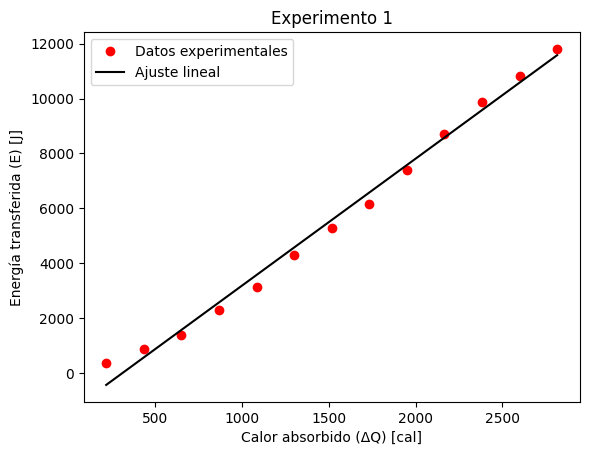
\includegraphics[scale=0.45]{exp1.png}
    \caption{Energía transferida vs Calor absorbido}
    \label{datos1}
\end{figure}
\begin{figure}[H]
    \centering
    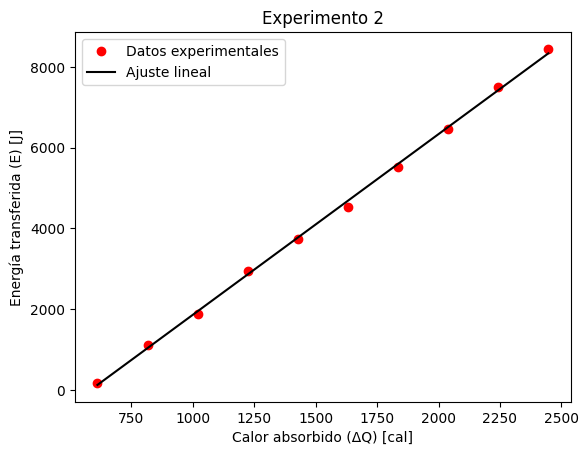
\includegraphics[scale=0.45]{exp2.png}
    \caption{Energía transferida vs Calor absorbido}
    \label{datos2}
\end{figure}
\begin{figure}[H]
    \centering
    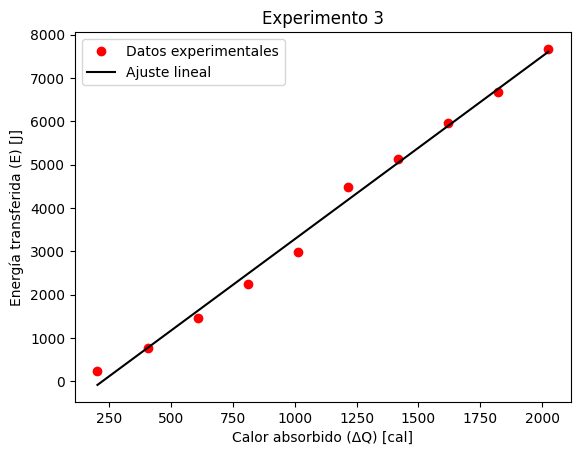
\includegraphics[scale=0.45]{exp3.png}
    \caption{Energía transferida vs Calor absorbido}
    \label{datos3}
\end{figure}
\begin{figure}[H]
    \centering
    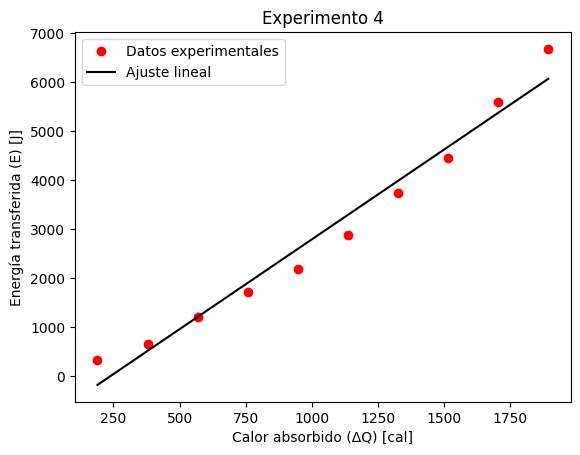
\includegraphics[scale=0.45]{exp4.png}
    \caption{Energía transferida vs Calor absorbido}
    \label{datos4}
\end{figure}

De estos resultados, se puede obtener por cada uno, el valor experimental de la constante $J$, y obtener un valor más certero considerando el promedio de todos los experimentos, a  continuación se presentan estos resultados;

\begin{table}[H]
\centering
\caption{Valores experimentales de la constante J y su error porcentual respecto del valor teorico}
\begin{tabular}{c|c|c}
\hline
\hline
\textbf{Experimento} & \textbf{J experimental $J/cal$} & \textbf{Error \%} \\
\hline
\hline
Exp 1 & $4.622 \pm 0.998$ & 10\% \\
\hline
Exp 2 & $4.472 \pm 0.999$ & 7\% \\
\hline
Exp 3 & $4.215 \pm 0.993$ & 1\% \\
\hline
Exp 4 & $3.660 \pm 0.971$ & 13\% \\
\hline
\end{tabular}
\end{table}

El experimento 2, presenta la menor desviación, incluso se puede observar en la gráfica \ref{datos2}, que el comportamiento de los datos es mucho más lineal, quiere decir, tiene más precisión que el resto de los experimentos; sin embargo, el resultado que mayor exactitud presenta es el experimento 3, (\textit{ver figura \ref{datos3}}).  \\

Por último se calcula el promedio de los valores experimentales, obteniendo así, el valor experimental concluyente de este experimento, y calculando el error porcentual respecto del valor considerado como correcto para esta constante.

\begin{equation}
 \begin{split}
    J_{exp} = 4.242 \pm 0.99 \,  J/cal\\
    J_{teorico} = 4.186 \, J/cal\\
    Error\% = 1.5
 \end{split}
\end{equation}

El valor obtenido de $J$ es bastante aceptable, con un error bajo, aun así es importante destacar los fallos que llevaron en el experimento a tener por ejemplo errores del $13\%$ cómo en el experimento 4.\\

La pérdida de calor, es un problema dentro del montaje experimental, ya que el calorímetro no está completamente aislado, por lo que es posible que ocurra una pérdida de calor hacia el entorno. Esta pérdida de calor no medido conduciría a una subestimación de la energía transferida en forma de calor y, por lo tanto, aumentaría el error en los cálculos de $J$.\\


Por otra parte, pueden ocurrir, variaciones en la resistencia, la resistencia utilizada para calentar el agua experimenta cambios en su resistencia interna debido a fluctuaciones en la temperatura ambiente o a un desgaste gradual, esto afectaría la cantidad de calor generada por la resistencia.\\

Pero el factor más significativo que genero un error en la práctica, fue la pérdida de energía eléctrica, ya que la energía suministrada al sistema fluctuaba en gran medida, y esto registrado por el voltímetro, el cual oscilaba al rededor de $\pm 20 V$, de la medida central, con la que se hizo los cálculos, esto puede ser debido a disipación de energía en los cables, conexiones o en la propia resistencia, debido al malgasto de las mismas, o el daño directo de la fuente de poder. Estas pérdidas no medidas reducirían la cantidad de energía transferida al agua y resultaran en un grave error de $J.$

No considerar otros factores de transferencia de energía en el análisis, es importante, ya que hay que tener en cuenta que la transferencia de energía en forma de calor no es el único mecanismo de transferencia de energía en el sistema. Pueden haber otras formas de transferencia de energía, como la conducción o la radiación, que no se están teniendo en cuenta en el experimento. Esta omisión puede introducir un error adicional en los resultados.\\

Aun así, el efectuar las mediciones más de una vez, bajo condiciones iniciales distintas, se logra disminuir el error, al tomar la media de los datos.\\

\subsection*{Cuestionario}

\begin{enumerate}
    \item Si se empleara un líquido con un calor específico de $0.25 cal/g C ^\circ$ en lugar de agua. El calor específico es una propiedad física de las sustancias y representa la cantidad de calor necesaria para elevar la temperatura de una unidad de masa de la sustancia en un grado Celsius. Un valor más bajo de calor específico significa que se requiere menos calor para elevar la temperatura de la sustancia en comparación con el agua. En el experimento, se basa en el supuesto de que el agua tiene un calor específico de $1 cal/g C ^\circ$, por lo que los cálculos y análisis se realizan en función de esta propiedad. Si se utiliza un líquido con un calor específico más bajo, se requeriría menos energía para elevar su temperatura en comparación con el agua. Esto significaría que la energía transferida y los resultados del experimento serían menores a los obtenidos en esta practica.

    \item Para evaluar hasta qué punto se satisfacen las condiciones indicadas en el modelo teórico, es necesario considerar varios aspectos:
    \begin{enumerate}
        \item \textbf{Calor específico del agua:} El modelo teórico asume que el agua tiene un calor específico de  $1 cal/g C ^\circ$. Es importante verificar experimentalmente si este valor se mantiene dentro de los límites aceptables. Para ello, se deben realizar mediciones precisas de la temperatura y la energía transferida y verificar si se obtienen resultados coherentes con las expectativas teóricas.
        \item  \textbf{Aislamiento térmico:} Dentro del modelo se asume un sistema de calorímetro perfectamente aislado, donde no hay intercambio de calor con el entorno. Es importante evaluar si el aislamiento del calorímetro utilizado en el experimento es efectivo y minimiza las pérdidas de calor hacia el entorno. Cualquier fuga de calor no deseada afectaría los resultados y la precisión de los cálculos.
        \item  \textbf{Transferencia de energía:} El marco teórico se basa en la transferencia de energía en forma de calor como el único mecanismo de transferencia de energía en el sistema. Es importante considerar si existen otros mecanismos de transferencia de energía, como la conducción o la radiación, y evaluar su impacto en los resultados experimentales.
        \item  \textbf{Condiciones experimentales:} Se deben evaluar las condiciones en las que se realizó el experimento para determinar si cumplen con las suposiciones y requisitos del modelo teórico. Esto incluye aspectos como la estabilización de la temperatura inicial, el control de la corriente eléctrica suministrada, la medición precisa de las variables relevantes y la 
        minimización de posibles fuentes de error.
    \end{enumerate}

    En resumen, para evaluar la satisfacción de las condiciones indicadas en el modelo teórico, es necesario comparar los resultados experimentales con las expectativas teóricas, identificar posibles desviaciones y fuentes de error, y realizar un análisis crítico de los datos obtenidos.
\end{enumerate}




\section{\small CONCLUSIONES}

En esta práctica experimental, se determinó la constante $J$ para la transferencia de calor utilizando un calorímetro. El valor obtenido para la constante $j$ fue de $4.24 J/cal$, con un error porcentual de $1.5\%$ en comparación con el valor teórico, lo cual brinda un valor bastante aceptable dentro de las fallas de la práctica experimental.\\

Es importante tener en cuenta que los errores de medición pueden haber contribuido a la discrepancia entre el valor experimental y el valor teórico esperado. Los errores de medición pueden deberse a diversos factores, como imprecisiones en las mediciones de masa, temperatura y fluctuaciones de la corriente eléctrica, así como posibles fugas de calor en el sistema.\\

A pesar de los errores de medición, se lograron cumplir los objetivos planteados en la práctica. Se pudo determinar la constante J, que es un parámetro fundamental para cuantificar la transferencia de calor en un sistema.\\

En conclusión, los resultados obtenidos en esta práctica proporcionan una estimación confiable de la constante J para la transferencia de calor en agua. Aunque se observó un pequeño error porcentual, brindando una comprensión más profunda del fenómeno físico estudiado y de las consideraciones experimentales asociadas.

\nocite{giancoli}
\nocite{montiel2015física}
\nocite{termal}
\nocite{ExperimentoJoule}
\bibliographystyle{elsarticle-num}
\bibliography{bib}

\end{multicols*}
\end{document}